\section{MD5}

MD5, designed by Ronald Rivest in 1991, is a widely used cryptographic hash function. Based on the Merkle-Damg\r{a}rd construction, this one-way function produces a 128-bit digest, usually presented in text format as a 32 digit hexadecimal number.  

While MD5 is past its prime and shall not be used for new applications, (as it is completely broken with regards to collisions, see Chapter~\ref{chap:security}) a lot of existing usages of MD5 are still reasonably robust and do not warrant emergency update. It remains a good example to understand how cryptographic hash functions based on the Merkle-Damg\r{a}rd construction work.

\subsection{MD5 Overview}
\cite{Att}
Here is how the MD5 algorithm operates on a given input M, where M is an arbitrary length bit string.
\begin{enumerate}
\item \emph{Padding}: The original message is padded so that the resulting length of $ M\vert \vert pad\lbrack 512\rbrack (\vert M\vert )$ is $512\cdot \vert M\vert_{512}$ where $\vert M\vert_{512}$ is a positive integer.

\item \emph{Partitioning}: The padded message $P= M\vert \vert pad\lbrack 512\rbrack (\vert M\vert )$ is split into $N=\vert M\vert_{512}$ consecutive blocs that are each 512 bits long:\\ $M_0, M_1,\ldots, M_{N−1}$.

\item \emph{Processing}: In order to hash a message that is made up of $N$ blocks, MD5 iterates through $N + 1$ states $IHV_i$, for $0 \le i \le N$, called \emph{intermediate hash values}. Each intermediate hash value $IHV_i$ is a tuple of four 32-bit words $(a_i, b_i, c_i, d_i)$. For $i = 0$, the tuple has a fixed public value, called \emph{initial value} $(IV)$:
$$(a_0,b_0,c_0,d_0) = (67452301_{16},efcdab89_{16},98badcfe_{16},10325476_{16}).$$

For $i = 1,2,\ldots,N$ the intermediate hash value $IHV_i$ is computed using MD5's compression function. This step is detailed in~\ref{sec:compressionMD5}:
$$IHV_i = \textsc{MD5Compress}(IHV_{i−1},M_{i−1}).$$

\item  \emph{Output}: The resulting hash value, $IHV_N$, is expressed as the concatenation of the hexadecimal byte strings of the four words $a_N , b_N , c_N , d_N$, converted back from their little-endian representation. An example of  $IHV_N$ could be:
 $$0123456789abcdeffedcba9876543210_{16}$$

\end{enumerate}
\subsection{MD5 Compression Function}\label{sec:compressionMD5}
The inputs of \textsc{MD5Compress} ($IVH_i$,$M_i$), producing the $i+1{th}$ intermediate hash value, are an intermediate hash value $IHV_{i}=(a,b,c,d)$ and a 512-bit block of the original message. The compression function iterates through 64 \emph{steps}, split into four consecutive \emph{rounds} of 16 steps each. Each step $t$ uses modular additions, a left rotation, a non-linear function $f_t$, an \emph{additional constant} $AC_t$ and a  \emph{rotation Constant} $RC_t$.

These constants are defined as follows:
\begin{equation}
AC_t = \lfloor 2^{32} \vert \sin(t+1)\vert \rfloor \mbox{, }  0\le t\le 64
\end{equation}
\begin{equation}
(RC_t, RC_{t+1}, RC_{t+2}, RC_{t+3})
\begin{cases}
(7, 12, 17, 22) & \mbox{ for } t = 0,4,8,12; \\
(5, 9, 14, 20) & \mbox{ for } t = 16, 20, 24, 28;\\
(4, 11, 16, 23) & \mbox{ for } t = 32, 36, 40, 44; \\
(6, 10, 15, 21) & \mbox{ for } t = 48,52,56,60; \\
\end{cases}
\end{equation}

The non-linear function $f_t$ depends on the round:

\begin{equation}
f_t(X,Y,Z)
\begin{cases}
F(X, Y, Z) = (X \wedge Y) \oplus (\overline{X} \wedge Z) & \mbox{ if } 0 \le t < 16; \\
G(X, Y, Z) = (Z \wedge X) \oplus (\overline{Z} \wedge Y) & \mbox{ if } 16 \le t < 32; \\
H(X, Y, Z) = X \oplus Y \oplus Z & \mbox{ if } 32 \le t < 48; \\
I(X, Y, Z) = Y \oplus (X \vee \overline{Z}) & \mbox{ if } 48 \le t < 64; \\
\end{cases}
\end{equation}

The 512-bit input message block $M_i$, of the original message, is divided into sixteen 32-bit long words $m_0,m_1,\ldots,m_{15}$ (using \emph{little endian} byte ordering). These words are then extended into sixty-four 32-bit words $W_t$ for $0 \le t < 64$:
\begin{equation}
W_t =
\begin{cases}
m_t & \mbox{ for } 0 \le t < 16; \\
m_{(1+5t)\mbox{ mod }16} & \mbox{ for } 16 \le t < 32; \\
m_{(5+3t)\mbox{ mod }16} & \mbox{ for } 32 \le t < 48; \\
m_{(7t)\mbox{ mod }16} & \mbox{ for } 48 \le t < 64; \\
\end{cases}
\end{equation}

\begin{figure}[!ht]
  \centering
  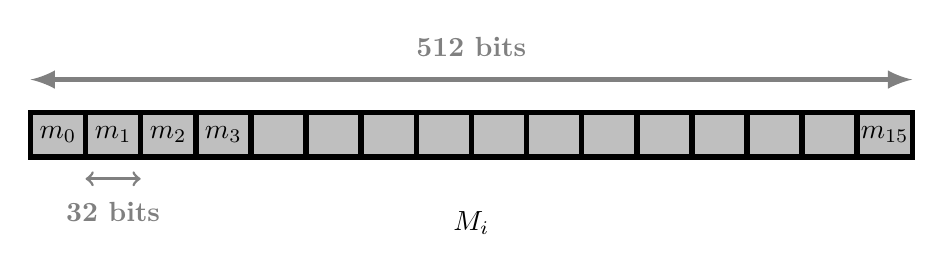
\begin{tikzpicture}[scale=1.4]

    \draw [fill=Gray!50, line width=2pt] (0,0) rectangle (0.5,0.4) node[pos=.5]{\textbf{$m_{0}$}};
    \draw [fill=Gray!50, line width=2pt] (0.5,0) rectangle (1,0.4) node[pos=.5]{\textbf{$m_{1}$}};
    \draw [fill=Gray!50, line width=2pt] (1,0) rectangle (1.5,0.4) node[pos=.5]{\textbf{$m_{2}$}};
    \draw [fill=Gray!50, line width=2pt] (1.5,0) rectangle (2,0.4) node[pos=.5]{\textbf{$m_{3}$}};
    \draw [fill=Gray!50, line width=2pt] (2,0) rectangle (2.5,0.4);
    \draw [fill=Gray!50, line width=2pt] (2.5,0) rectangle (3,0.4);
    \draw [fill=Gray!50, line width=2pt] (3,0) rectangle (3.5,0.4);
    \draw [fill=Gray!50, line width=2pt] (3.5,0) rectangle (4,0.4);
    \draw [fill=Gray!50, line width=2pt] (4,0) rectangle (4.5,0.4);
    \draw [fill=Gray!50, line width=2pt] (4.5,0) rectangle (5,0.4);
    \draw [fill=Gray!50, line width=2pt] (5,0) rectangle (5.5,0.4);
    \draw [fill=Gray!50, line width=2pt] (5.5,0) rectangle (6,0.4);
    \draw [fill=Gray!50, line width=2pt] (6,0) rectangle (6.5,0.4);
    \draw [fill=Gray!50, line width=2pt] (6.5,0) rectangle (7,0.4);
    \draw [fill=Gray!50, line width=2pt] (7,0) rectangle (7.5,0.4);
    \draw [fill=Gray!50, line width=2pt] (7.5,0) rectangle (8,0.4) node[pos=.5]{\textbf{$m_{15}$}};

    \draw [<->, >=latex, line width=2pt, color=Gray] (0,0.7) -- (8,0.7);
    \draw [<->, line width=1pt, color=Gray] (0.5,-0.2) -- (1,-0.2);

    \node [align=center, color=Gray] at (4,1){\textbf{512 bits}};
    \node [align=center, color=Gray] at (0.75,-0.5){\textbf{32 bits}};
    \node [align=center] at (4,-0.6){\textbf{$M_i$}};
    
  \end{tikzpicture}
  \caption{\label{fig:B}$M_i$ is divided into sixteen 32-bit words.}
\end{figure}

For each step t, the compression function uses a working state, consisting of four 32-bit words $Q_t, Q_{t-1}, Q_{t-2}$ and $Q_{t-3}$ and computes a new word of the working state $Q_{t+1}$. The initial value of the working state is  $(Q_0, Q_{-1}, Q_{-2},Q_{-3}) = (b,c,d,a)$.

For $t=0,1,\ldots,63$, the subsequent working state $Q_{t+1}$ is computed as follows:
\begin{equation}
\begin{aligned}
  &F_t = f_t(Q_t, Q_{t-1}, Q_{t-2}); \\
  &T_t = F_t + Q_{t-3} + AC_t + W_t; \\
  &R_t = RL(T_t,RC_t); \\
  &Q{t_+1} = Q_t +R_t; \\
\end{aligned}
\end{equation}

Once all the steps have been computed, the resulting state words are added to the input intermediate hash values, and returned as output:
\begin{equation}
MD5Compress(IHV_{i}, M_i) = (a + Q_{61}, b + Q_{64}, c + Q_{63}, d + Q_{62}).
\end{equation}

\subsection{MD5 Algorithm}~\label{section:md5}
The pseudo-code for the MD5 algorithm is presented in Algorithm~\ref{algo:md5}.
\begin{algorithm}[H]
\caption{MD5(x)}
\label{algo:md5}
\begin{algorithmic}[1]
\State{\textbf{external procedures} MD5-\textsc{pad}}
\State{Define $RC\lbrack 64\rbrack$: the array of rotation constants.}
\State{Define $AC\lbrack 64\rbrack$: the array of additional constants.}
\State{$RC\lbrack 0{\ldots}15\rbrack \gets \{7, 12, 17, 22,  7, 12, 17, 22,  7, 12, 17, 22,  7, 12, 17, 22\}$}
\State{$RC\lbrack 16{\ldots}31\rbrack \gets \{5,  9, 14, 20,  5,  9, 14, 20,  5,  9, 14, 20,  5,  9, 14, 20\}$}
\State{$RC\lbrack 32{\ldots}47\rbrack \gets \{4, 11, 16, 23,  4, 11, 16, 23,  4, 11, 16, 23,  4, 11, 16, 23\}$}
\State{$RC\lbrack 48{\ldots}63\rbrack \gets \{6, 10, 15, 21,  6, 10, 15, 21,  6, 10, 15, 21,  6, 10, 15, 21\}$}

\For{$i \gets 0$ to $63$ }
\State{$AC\lbrack i\rbrack \gets \lfloor 2^{32} \vert \sin(t+1)\vert \rfloor$}
\EndFor{}

\Comment{Initialise variables}
\State{$a_0 \gets \mbox{0x67452301}$}
\State{$b_0 \gets \mbox{0xefcdab89}$}
\State{$c_0 \gets \mbox{0x98badcfe}$}
\State{$d_0 \gets \mbox{0x10325476}$}

\State{$M_1 \vert \vert M_2 \vert \vert \ldots \vert \vert M_N \gets$ MD5-\textsc{pad} (x), where each  $M_i$ is a 512-bit block.}

\Comment{Loop through all $N$ message blocs to hash.}
\For{$i \gets 1$ to $N$ }
\State{Define $W\lbrack 16\rbrack$: the array of 32-bit words in $M_i$. }
\State{$M_i = W\lbrack 0\rbrack \vert \vert W\lbrack 1\rbrack \vert \vert \ldots vert \vert W\lbrack 15\rbrack$.}

\Comment{Initial values}
\State{$a \gets a_0$}
\State{$b \gets b_0$}
\State{$c \gets c_0$}
\State{$d \gets d_0$}

\Comment{Iterate through the 64 steps of the compression function}
\For{$t \gets 0$ to $63$ }
\If{$0\le i \le 15$}
\Comment{$f_t$ is F and $W_t$ is $m_t$}
\State{$f \gets (b \wedge c) \oplus (\overline{b} \wedge d)$}
\State{$g \gets t$}

\ElsIf{$16\le i \le 31$}
\Comment{$f_t$ is G and $W_t$ is $m_{1+5t}$}
\State{$f \gets (d \wedge b) \oplus (\overline{d} \wedge c)$}
\State{$g \gets (5*t+1) \mod{16}$}

\ElsIf{$32\le i \le 47$}
\Comment{$f_t$ is H and $W_t$ is $m_{5+3t}$}
\State{$f \gets b \oplus c \oplus d$}
\State{$g \gets (3*t+5) \mod{16}$}

\ElsIf{$48\le i \le 63$}
\Comment{$f_t$ is I and $W_t$ is $m_{7t}$}
\State{$f \gets c \oplus (b \vee \overline{d})$}
\State{$g \gets (7*t) \mod{16}$}
\EndIf{}

\State{$temp \gets d$}
\State{$d \gets c$}
\State{$c \gets b$}
\State{$b \gets ((a + f + AC\lbrack t \rbrack + W\lbrack g \rbrack)) +b $}
\State{$a \gets temp$}
\EndFor{}

\Comment{Once all the steps have been computed, the resulting state words are added to the input intermediate hash values}
\State{$a_0 \gets a_0 + a$}
\State{$b_0 \gets b_0 + b$}
\State{$c_0 \gets c_0 + c$}
\State{$d_0 \gets d_0 + d$}

\EndFor{}

\Return{$digest \gets a_0 \vert \vert b_0 \vert \vert c_0 \vert \vert d_0 \vert \vert H_4$}

\Comment{Return output as little endian}
\end{algorithmic}
\end{algorithm}
